\documentclass[hide notes,intlimits]{beamer}


\mode<presentation>
{
  \usetheme[footline]{UAFshade}
  \setbeamercovered{transparent}
}

% load packages
\usepackage[english]{babel}
\usepackage[latin1]{inputenc}
\usepackage[T1]{fontenc}
\usepackage{lmodern}
\usepackage[multidot]{grffile}

\usepackage{tikz}
\usetikzlibrary{shapes,arrows,shadows, calc}

\definecolor{dark red}{HTML}{E41A1C}
\definecolor{dark green}{HTML}{4DAF4A}
\definecolor{dark violet}{HTML}{984EA3}
\definecolor{dark blue}{HTML}{084594}
\definecolor{dark orange}{HTML}{FF7F00}
\definecolor{light blue}{HTML}{377EB8}
\definecolor{light red}{HTML}{FB9A99}
\definecolor{light violet}{HTML}{CAB2D6}

\definecolor{uaf red}{HTML}{E41A1C}
\definecolor{uaf blue}{HTML}{377EB8}
\definecolor{uaf green}{HTML}{4DAF4A}
\definecolor{uaf violet}{HTML}{984EA3}
\definecolor{uaf orange}{HTML}{FF7F00}
\setbeamercolor{boxed}{fg=black,bg=uaf yellow}

\graphicspath{{figures/}}

\setbeamerfont{caption}{size=\scriptsize}

% code adapted from http://tex.stackexchange.com/a/11483/3954

% some parameters for customization
\def\shadowshift{3pt,-3pt}
\def\shadowradius{6pt}

\colorlet{innercolor}{black!60}
\colorlet{outercolor}{gray!05}

% this draws a shadow under a rectangle node
\newcommand\drawshadow[1]{
    \begin{pgfonlayer}{shadow}
        \shade[outercolor,inner color=innercolor,outer color=outercolor] ($(#1.south west)+(\shadowshift)+(\shadowradius/2,\shadowradius/2)$) circle (\shadowradius);
        \shade[outercolor,inner color=innercolor,outer color=outercolor] ($(#1.north west)+(\shadowshift)+(\shadowradius/2,-\shadowradius/2)$) circle (\shadowradius);
        \shade[outercolor,inner color=innercolor,outer color=outercolor] ($(#1.south east)+(\shadowshift)+(-\shadowradius/2,\shadowradius/2)$) circle (\shadowradius);
        \shade[outercolor,inner color=innercolor,outer color=outercolor] ($(#1.north east)+(\shadowshift)+(-\shadowradius/2,-\shadowradius/2)$) circle (\shadowradius);
        \shade[top color=innercolor,bottom color=outercolor] ($(#1.south west)+(\shadowshift)+(\shadowradius/2,-\shadowradius/2)$) rectangle ($(#1.south east)+(\shadowshift)+(-\shadowradius/2,\shadowradius/2)$);
        \shade[left color=innercolor,right color=outercolor] ($(#1.south east)+(\shadowshift)+(-\shadowradius/2,\shadowradius/2)$) rectangle ($(#1.north east)+(\shadowshift)+(\shadowradius/2,-\shadowradius/2)$);
        \shade[bottom color=innercolor,top color=outercolor] ($(#1.north west)+(\shadowshift)+(\shadowradius/2,-\shadowradius/2)$) rectangle ($(#1.north east)+(\shadowshift)+(-\shadowradius/2,\shadowradius/2)$);
        \shade[outercolor,right color=innercolor,left color=outercolor] ($(#1.south west)+(\shadowshift)+(-\shadowradius/2,\shadowradius/2)$) rectangle ($(#1.north west)+(\shadowshift)+(\shadowradius/2,-\shadowradius/2)$);
        \filldraw ($(#1.south west)+(\shadowshift)+(\shadowradius/2,\shadowradius/2)$) rectangle ($(#1.north east)+(\shadowshift)-(\shadowradius/2,\shadowradius/2)$);
    \end{pgfonlayer}
}

% create a shadow layer, so that we don't need to worry about overdrawing other things
\pgfdeclarelayer{shadow} 
\pgfsetlayers{shadow,main}

\newsavebox\mybox
\newlength\mylen

\newcommand\shadowimage[2][]{%
\setbox0=\hbox{\includegraphics[#1]{#2}}
\setlength\mylen{\wd0}
\ifnum\mylen<\ht0
\setlength\mylen{\ht0}
\fi
\divide \mylen by 120
\def\shadowshift{\mylen,-\mylen}
\def\shadowradius{\the\dimexpr\mylen+\mylen+\mylen\relax}
\begin{tikzpicture}
\node[anchor=south west,inner sep=0] (image) at (0,0) {\includegraphics[#1]{#2}};
\drawshadow{image}
\end{tikzpicture}}

\newcommand\shadowimagec[3][]{%
\setbox0=\hbox{\includegraphics<#1>[#2]{#3}}
\setlength\mylen{\wd0}
\ifnum\mylen<\ht0
\setlength\mylen{\ht0}
\fi
\divide \mylen by 120
\def\shadowshift{\mylen,-\mylen}
\def\shadowradius{\the\dimexpr\mylen+\mylen+\mylen\relax}
\begin{tikzpicture}
\node[anchor=south west,inner sep=0] (image) at (0,0) {\includegraphics<#1>[#2]{#3}};
\drawshadow{image}
\end{tikzpicture}}


\newenvironment{transbox}[1][]{%
\begin{tikzpicture}
\node[drop shadow,rounded corners,text width=\textwidth,fill=white, fill opacity=#1,text opacity=1] \bgroup
}{
\egroup;\end{tikzpicture}} 

\newenvironment{transbox-tight}{%
\begin{tikzpicture}
\node[drop shadow,rounded corners,fill=uaf yellow, fill opacity=0.75,text opacity=1] \bgroup
}{
\egroup;\end{tikzpicture}} 


% title page
\title[] % (optional, use only with long paper titles)
{High resolution modeling of the Greenland Ice Sheet}

\subtitle{using the Parallel Ice Sheet Model (PISM)}


\author[Aschwanden, Fahnestock, Truffer] % (optional, use only with lots of authors)
{}
% - Give the names in the same order as the appear in the paper.
% - Use the \inst{?} command only if the authors have different
%   affiliation.

\institute[Geophysical Institute] % (optional, but mostly needed)
{}
% - Use the \inst command only if there are several affiliations.
% - Keep it simple, no one is interested in your street address.

\titlegraphic{\vskip-0.5cm\includegraphics[width=\textwidth]{gris-nw-speed-exp-600m}}

\date{}

\begin{document}

% define what is shown at the beginning of each section
\AtBeginSection[]
{
  \begin{frame}<handout:0>
    \frametitle{Outline}
   \tableofcontents[currentsection,subsectionstyle=hide/hide/hide]
  \end{frame}
}

% define what is shown at the beginning of each subsection
\AtBeginSubsection[]
{
 \begin{frame}<beamer>
  \frametitle{Outline}
   \tableofcontents[currentsection,currentsubsection]
 \end{frame}
}

\setbeamertemplate{background canvas}
  {
     \tikz{\node[inner sep=0pt,opacity=1.0] {\includegraphics[width=\paperwidth]{uaf_beamer_shade_bg}};}
} 


% insert titlepage
\begin{frame}
  \titlepage
\end{frame}

\setbeamertemplate{background canvas}
{
%
} 

\setbeamertemplate{background canvas}
  {
     \tikz{\node[inner sep=0pt,opacity=1.0] {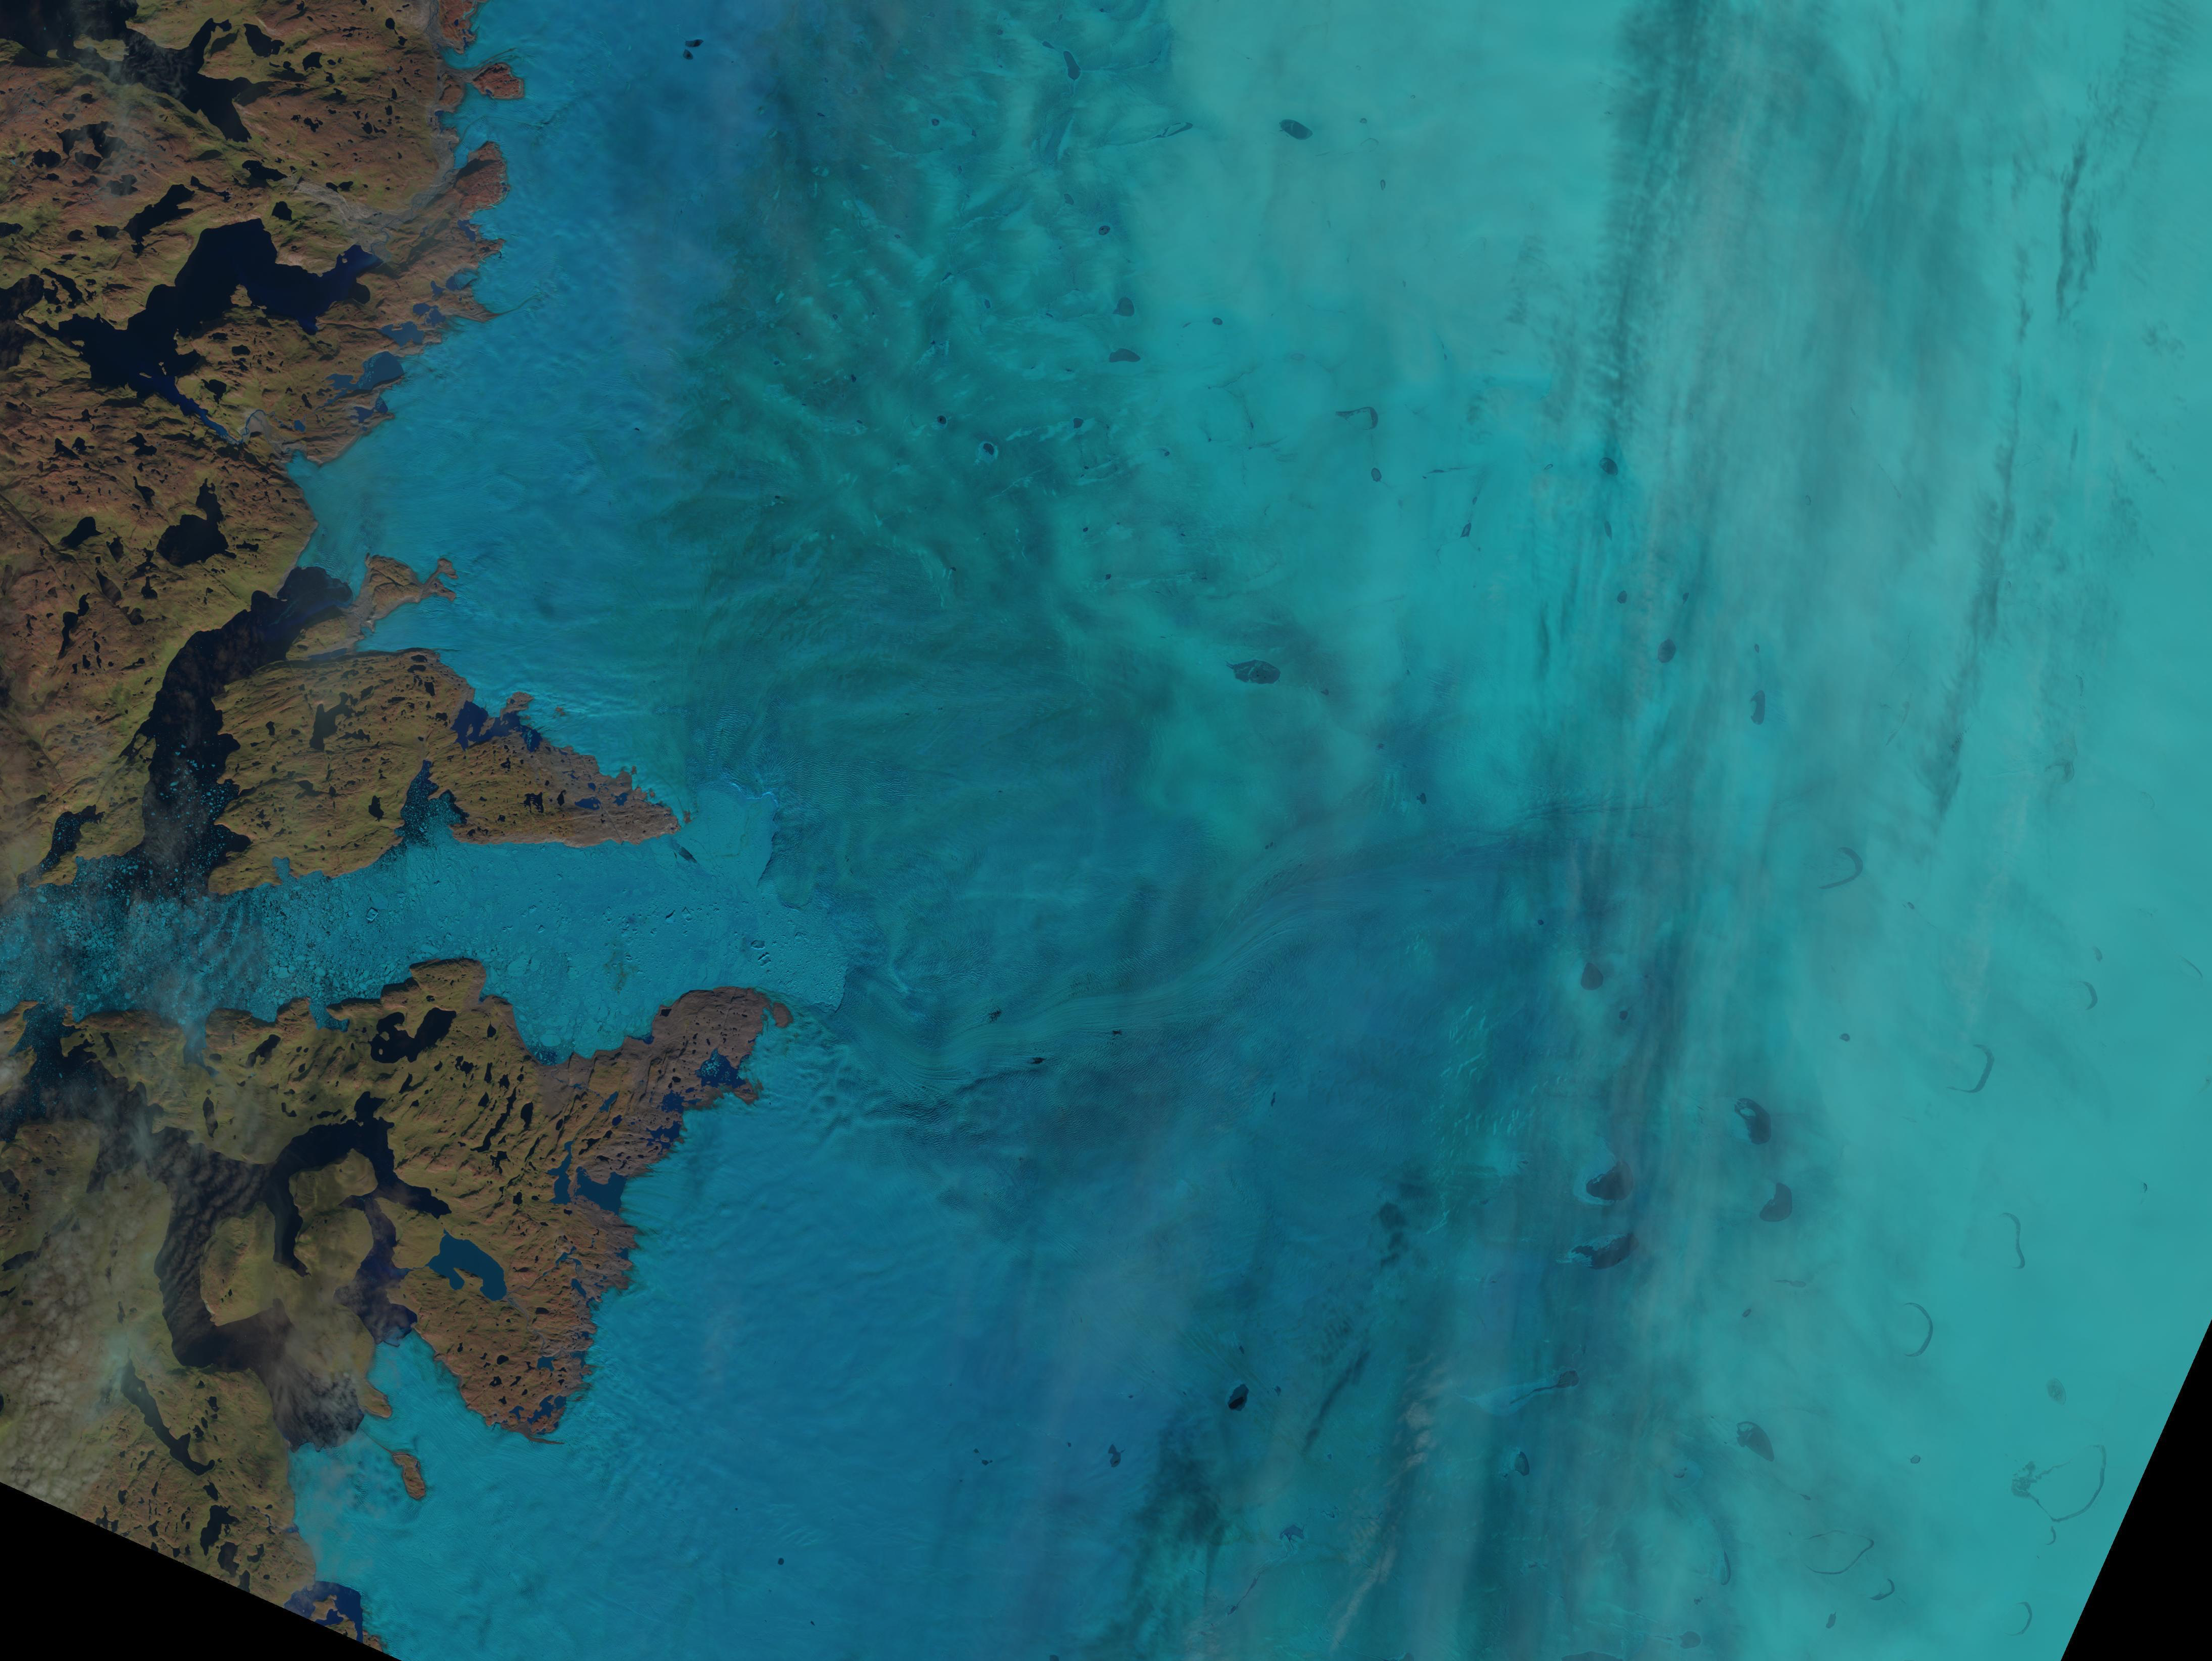
\includegraphics[width=\paperwidth,height=\paperheight]{jakobshavn_landsat8}};}
} 

\begin{frame}[plain]
  \vspace{-3em}
  \begin{transbox}[0.4]
    \begin{itemize}
    \item Over the past decades, the Greenland Ice Sheet (GrIS) has been loosing mass at an accelerating rate, thereby raising global mean sea level
    \end{itemize}
  \end{transbox}
\end{frame}

\begin{frame}[plain]
  \vspace{-3em}
  \begin{transbox}[0.4]
    \begin{itemize}
    \item Ice discharge to the ocean mainly occurs through Greenland's 200+ outlet glaciers
    \end{itemize}
  \end{transbox}
\end{frame}

\begin{frame}[plain]
  \vspace{-3em}
  \begin{transbox}[0.4]
    \begin{itemize}
    \item Outlet glaciers are fast-flowing ($>$200\,m/yr) topographically-controlled features terminating in narrow fjords $\sim\le$10\,km wide.
    \end{itemize}
  \end{transbox}
\end{frame}

\setbeamertemplate{background canvas}
{
%
} 

\begin{frame}{Flow speeds}
\vspace{-0.74em}
  \begin{columns}
    \column[c]{5cm}
    \begin{figure}
      \includegraphics[width=\textwidth]{greenland-obs-overview}
    \end{figure}
    \column[c]{5cm}
    \only<1>{Jakobshavn Isbr{\ae}}
    \includegraphics<1>[width=\textwidth]{jakobshavn-obs-nogate}
    \only<1>{\\ {} }
  \end{columns}
\end{frame}


\setbeamertemplate{background canvas}
  {
     \tikz{\node[inner sep=0pt,opacity=.3] {\includegraphics[height=\paperheight,width=\paperwidth]{grn_iss}};}
} 


\begin{frame}[plain]
  \begin{transbox}[0.8]
    \begin{block}{We note}
      \begin{itemize}
      \item any credible modeling effort must be able to explain this variability
      \item model resolution must be high enough to capture outlet glaciers
      \item Glaciology 100: ice thickness is a leading order constraint on flow
      \end{itemize}
    \end{block}
  \end{transbox}
\end{frame}


\setbeamertemplate{background canvas}
{
%
} 


\begin{frame}
  \begin{block}{Until recently models were not able to capture outlet glacier flow due to}
    \begin{itemize}
    \item insufficient model resolution
    \item insufficient input data set resolution
    \end{itemize}
  \end{block}
\end{frame}

\begin{frame}
  \begin{block}{Progress was made due to}
    \begin{itemize}
    \item model improvements (parallelism, efficient meshing, etc)
    \item large scale data collection efforts to increase input data set resolution
    \end{itemize}
  \end{block}
\end{frame}



\begin{frame}{Zoom in to Jakobshavn Isbr{\ae}}
  \begin{figure}
    \small{Bamber (2001) \hspace{5em} Morlighem (2014)}
    \includegraphics[width=12cm]{jako_bed}
 \end{figure}
\end{frame}


\begin{frame}{NASA Operation IceBridge}
  \begin{columns}
    \column[c]{8cm}
    \begin{figure}
      \small{Bamber (2001) \hspace{4em} Morlighem (2014)}
      \includegraphics[height=7.5cm]{greenland_bed}
    \end{figure}
    \column[c]{4cm}
    \begin{itemize}
    \item from 5\,km to 150\,m horizontal grid resolution
    \end{itemize}
  \end{columns}
\end{frame}

\begin{frame}{NASA Operation IceBridge}
  \begin{figure}
    \includegraphics[height=2.5cm]{nasa-logo} \qquad
    \includegraphics[height=2.5cm]{oib} \qquad
    \includegraphics[height=2.5cm]{1000-dollar-bills}
  \end{figure}
  \begin{itemize}
  \item do NASA's OIB million\$ really make ice sheet models better?
  \item use your favorite high resolution ice sheet model to find out
\end{itemize}
\end{frame}


\begin{frame}{Validation metrics: flow through flux gates}
  \vspace{-1em}
  \begin{columns}
    \column[c]{4cm}
    \begin{figure}
      \includegraphics<1>[width=3cm]{upernavik-gate-zoom}
    \end{figure}
    \begin{figure}
      \includegraphics<1>[width=4cm]{Kong_Oscar_Gletscher_velsurf_normal_profile_250m_greenland_2008-2009_grid_mo14_flow_sel_green}
    \end{figure}
    \column[c]{7cm}
    \begin{figure}
      \includegraphics<1>[height=7.5cm]{greenland-gates-29}
    \end{figure}
  \end{columns}
\end{frame}


\begin{frame}{Validation metrics: flow through flux gates}
  \vspace{-1em}
  \begin{columns}
    \column[c]{4cm}
    \begin{figure}
      \includegraphics<1>[width=3cm]{upernavik-gate-zoom}
    \end{figure}
    \begin{figure}
      \includegraphics<1>[width=4cm]{Kong_Oscar_Gletscher_velsurf_normal_profile_250m_greenland_2008-2009_grid_mo14_flow_sel_green}
    \end{figure}
    \column[c]{7cm}
    \begin{block}{Metrics of success}
      \begin{itemize}
      \item assess model performance by comparing observed and simulated surface velocities along cross-flow profiles of 29  outlet glaciers
      \item quantify model's ability to capture the spatial variation in flow structure using \vspace{-.75em}
        \begin{itemize}
        \item the Pearson $r$ correlation coefficient and 
        \item the r.m.s. difference
        \end{itemize}
        between observations and simulations along the 29 profiles
      \item evaluate every 250\,m \alert{$\Rightarrow$ gates as shapefiles available on github}
      \end{itemize}
    \end{block}
  \end{columns}
\end{frame}


\begin{frame}{Model setup}
  \includegraphics[width=4cm]{pism-logo}
  \begin{itemize}
  \item this study is not about PISM
  \item any ISM capable of <1\,km grid resolution will do
  \item enthalpy field from a paleo-climate initialization
  \item calculate diagnostic velocity fields that correspond to a given geometry using flux correction method
  \end{itemize}
\end{frame}




\begin{frame}{Best simulation}
  \includegraphics[height=8cm]{greenland-overview-3}
\end{frame}

\begin{frame}{Role of model resolution}
  \includegraphics[width=\textwidth]{jakobshavn-beds}
\end{frame}

\begin{frame}{Role of model resolution}
  \begin{figure}
    \includegraphics[height=6cm]{grid-resolution-4}
  \end{figure}
\end{frame}


\begin{frame}{Role of ice thickness}
  \begin{figure}
    \includegraphics<1>[width=\textwidth]{nw-coast-1-4500m-ba2001-01}
    \includegraphics<2>[width=\textwidth]{nw-coast-1-4500m-mo2014-01}
    \includegraphics<3>[width=\textwidth]{nw-coast-1-600m-ba2001-01}
    \includegraphics<4>[width=\textwidth]{nw-coast-1-600m-mo2014-01}
    \\[1em]
    \only<1>{low model and low data set resolution}
    \only<2>{low model and high  data set resolution}
    \only<3>{high model and low data set resolution}
    \only<4>{high model and high data set resolution}
  \end{figure}
\end{frame}

\begin{frame}{Role of ice thickness}
  \begin{figure}
    \includegraphics<1>[width=\textwidth]{nw-coast-1-600m-mo2014-01}
  \end{figure}
      \begin{itemize}
        \item only {\bf high} \alert{model} and \alert{data} set resolution result in outlet glacier flow
      \end{itemize}
\end{frame}


\begin{frame}{What really matters}
  \begin{enumerate}
    \item an accurate map of subglacial topography
    \item a stress regime in which viscous membrane stresses are part of the balance with basal sliding resistance
    \item an energy-conservation-driven basal stress model derived (conceptually) from a model of a wet, pressurized, deformable basal layer
    \item  high model resolution over all areas of the ice sheet where sliding is possible and/or steep/rough basal topography exists
  \end{enumerate}
\end{frame}


\begin{frame}{Conclusions}
  \begin{itemize}
    \item first time that the general flow patterns are captured for the {\bf right} reason
    \item for isbr{\ae}-type glaciers ice thickness matters the most, subglacial hydrology comes later
    \item this is very encouraging
    \item opens the door for prognostic simulations using simple models of subglacial hydrology
  \end{itemize}
\end{frame}



\begin{frame}{Final Remarks}
  \begin{itemize}
    \item ice thickness mapping by NASA's OIB and similar efforts are paying off big time
    \item similar efforts are suggested for Antarctica
  \end{itemize}
\end{frame}


\begin{frame}{Final Remarks}
\begin{columns}
  \column[c]{3cm}
  \begin{figure}
    \includegraphics[width=1.75cm]{pandoras-box}
  \end{figure}
  \column[c]{8cm}
  The days of coarse ($>$1\,km) resolution Greenland models are over
\end{columns}
\end{frame}





\end{document}
